\documentclass{article}
\usepackage{hyperref}
\usepackage[margin=0.5in]{geometry}
\usepackage{amsmath}
\usepackage{graphicx}
\usepackage[bottom]{footmisc}
\usepackage{lastpage}
\usepackage{fancyhdr}
\usepackage{float}
\usepackage{tabularx}

\graphicspath{ {./assets/} }

\pagestyle{fancy}
\fancyhf{} % clear existing header/footer entries
% Place Page X of Y on the right-hand
% side of the footer
\fancyfoot[R]{Yang \thepage \hspace{1pt} of \pageref{LastPage}}
\renewcommand{\headrulewidth}{0pt}

\title{PHYSIOL 578: HW 2.3\footnotetext{U-M GPT was used to help draft and refine the answers.}}
\author{Jack Yang \\ \href{mailto:yhyunjoo@umich.edu}{yhyunjoo@umich.edu}}

\begin{document}
\maketitle
\thispagestyle{fancy}

\section{
    You are studying two newly identified G-protein coupled Receptors (GPCRs): GPCR-A and GPCR-B.
    GPCR-A and GPCR-B bind and activate different heterotrimeric G-proteins.
    You treat cell lines that express either GPCR-A or GPCR-B with their respective agonist and observe that intracellular cAMP concentration changes as summarized in Table~\ref{tab:1}:
}

\begin{table}[h]
    \centering
    \begin{tabular}{|l|c|c|}
        \hline
        & \multicolumn{2}{c|}{\textbf{Intracellular cAMP concentration}} \\
        \cline{2-3}
        & \textbf{GPCR-A expressing cell line} & \textbf{GPCR-B expressing cell line} \\
        \hline
        \textbf{Agonist A for GPCR-A} & Increase & No change \\
        \hline
        \textbf{Agonist B for GPCR-B} & No change & Decrease \\
        \hline
    \end{tabular}
    \caption{changes in intracellular cAMP concentrations}
    \label{tab:1}
\end{table}

\subsection*{
    A. (1 point)
    Based on these observations and what you learned in PHYSIOL578,
    what type of heterotrimeric G-protein (Gs, Gi or Gq) does GPCR-A interact with to mediate its signaling?
    What about GPCR-B?
}
GPCR-A seems to interact with Gs since Gs activation stimulates adenylyl cyclase, increasing cAMP.
On the other hand, since agonist for GPCR-B decreased cAMP concentration, it likely interacts with Gi.

\subsection*{
    B. (1 points)
    To investigate within GPCR-A and GPCR-B the agonist binding domain and the G protein-GPCR interacting domain,
    you generate 3 chimeric receptors as shown in Figure~\ref{fig:1}.
    You treat the 3 cell lines with either agonist A or B, and see the following changes in intracellular cAMP concentrations in Table~\ref{tab:2}.
    Based on these observations and what you learned in PHYSIOL578,
    which domains are \textit{\textbf{potentially}} involved in agonist binding and which domains are involved in G protein-GPCR interaction?
    When describing the domain, please use E1, E2..E4 to describe extracellular domains;
    C1, C2…C4 to describe cytosolic domains;
    and helix 1 to 7 to describe transmembrane domains.
}

\begin{figure}[H]
    \centering
    \caption{Chimeric Receptors}
    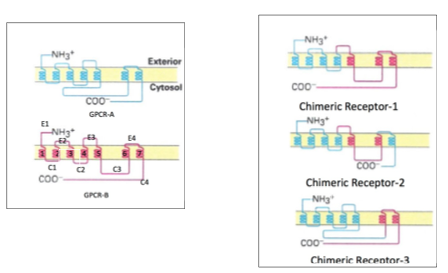
\includegraphics[width=0.5\textwidth]{fig1.png}
    \label{fig:1}
\end{figure}

\begin{table}[h]
    \centering
    \begin{tabular}{|l|c|c|c|}
        \hline
        & \multicolumn{3}{c|}{\textbf{cAMP}} \\
        \cline{2-4}
        & \textbf{\begin{tabular}[c]{@{}c@{}}Chimeric Receptor-1\\ expressing cell line\end{tabular}}
        & \textbf{\begin{tabular}[c]{@{}c@{}}Chimeric Receptor-2\\ expressing cell line\end{tabular}}
        & \textbf{\begin{tabular}[c]{@{}c@{}}Chimeric Receptor-3\\ expressing cell line\end{tabular}} \\
        \hline
        \textbf{Agonist A} & No change & Decrease & No change \\
        \hline
        \textbf{Agonist B} & Decrease & No change & Increase \\
        \hline
    \end{tabular}
    \caption{changes in intracellular cAMP concentrations}
    \label{tab:2}
\end{table}

Since chimeric receptor 1 did not see any activity from agonist A,
we deduce that one of its domains from GPCR-B is responsible for binding:
E3, E4, C3, C4, helices 5, 6, and 7.
Since chimeric receptor 2 saw activity from agonist A,
we deduce that one of its domains from GPCR-A is responsible for binding:
E1, E2, E4, C1, C2, C4, helices 1, 2, 3, 4, 7.
Since chimeric receptor 3 saw no activity from agonist A,
we deduce that one of its domains from GPCR-B is responsible for binding:
E4, C4, helices 6 and 7.
Together, these leave E4, C4, and helix 7 as possible candidates.
However, we know that the agonist must bind in extracellular space,
so E4 and/or helix 7 must be the binding domain.

We can confirm the results with whether agonist B induced activity in the chimeric receptors.

We go through the same process for the domains involved in G-protein and GPCR interaction.
Since chimeric receptor 2 saw a decrease in cAMP with agonist A,
we deduce that one of its domains from GPCR-B is responsible for the interaction:
E3, C3, and helices 5 and 6.
Since chimeric receptor 1 saw a decrease in cAMP with agonist B,
we deduce that one of its domains from GPCR-B is responsible for the interaction:
E3, E4, C3, C4, helices 5, 6, and 7.
Since chimeric receptor 3 saw an increase in cAMP with agonist B,
we deduce that one of its domains from GPCR-A is responsible for the interaction:
E1, E2, E3, C1, C2, C3, helices 1 through 5.
Together, these leave E3, C3, and helix 5 as the only possible domain.
However, we know that the G-protein and GPCR interact in the cytosol,
so C3 and/or helix 5 must be the interaction domain.

\subsection*{
    C. (1 points)
    What effect will adding pertussis toxin have on cellular cAMP levels when added in addition to agonist A or to agonist B for all 5 cell lines
    (cells expressing GPCR-A, GPCR-B, Chimeric Receptor-1, 2, or 3).
    Feel free to use a table format.
}

\begin{table}[h]
    \centering
    \begin{tabularx}{\linewidth}{|l|*{5}{>{\centering\arraybackslash}X|}}
        \hline
        & \multicolumn{5}{c|}{\textbf{cAMP}} \\
        \cline{2-6}
        & \textbf{GPCR-A expressing cell line}
        & \textbf{GPCR-B expressing cell line}
        & \textbf{Chimeric Receptor-1 expressing cell line}
        & \textbf{Chimeric Receptor-2 expressing cell line}
        & \textbf{Chimeric Receptor-3 expressing cell line} \\
        \hline
        \textbf{Agonist A} & No effect due to Gs & No effect due to inactive GPCR & No effect due to inactive GPCR & Increase & No effect due to inactive GPCR \\
        \hline
        \textbf{Agonist B} & No effect due to inactive GPCR & Increase & Increase & No effect due to inactive GPCR & No effect due to Gs \\
        \hline
    \end{tabularx}
\end{table}


Pertussis toxin only affects Gi by keeping it in inactive state.
This means whichever receptors have GPCR-B interaction domain
and decrease cAMP concentration by activating Gi will see an increase in cAMP
since the inhibition of adenylyl cylcase is removed.

\end{document}